\begin{tatb}
 \chapter{Revisiting the TA+/TB- hypothesis: interfacial potentials in periodic boundaries~}
 \hyperlink{toc}{Return to TOC}
  \section{\label{ch6:sec0:level1}Preface~}
  
   Disclaimer: this chapter is subject to additional changes as it is not yet published.
  
   The free energy change for transferring an ion across chemical interfaces includes a surface potential contribution. This potential has two parts: 1) the actual 
   surface or contact potential between two immiscible phases and 2) a solvent-specific local potential around the ion. In periodic boundary calculations without 
   an explicit vapor or vacuum region, the second potential still contributes to the solvation free energy and enthalpy. Simulation results therefore fall on an 
   unphysical, intermediate thermodynamic scale which needs to be adjusted to remove 2) or add 1) in order to properly facilitate comparison with one of the two
   major branches of single-ion quantities. Using ionic parameters which have not been optimized to fit one of these scales and which approach the size limit of the 
   tetraphenylarsonium and tetraphenylborate ions, I illustrate that the intermediate free energy scale is the one which predicts the $\approx$20 kcal/mol hydration
   asymmetry in water\cite{wipff1999tatb,wipff2000tatb,wipff2001tatb}. These large ions are otherwise assumed to have the same solvation free energy due to ample 
   charge screening effects\cite{marcus1987tatb}. The bulk or \emph{intrinsic} free energy scale (removing 2) above) predicts a 2-4 kcal/mol deviation from this 
   ideal behavior. I have also made predictions of the deviation in dimethyl sulfoxide and 1,2-dichloroethane, covering a broad spectrum of dielectric constants
   (10 to 80). I find dimethyl sulfoxide satisfies this condition as well while 1,2-dichloroethane violates it thanks to a large, anion favoring asymmetry. My 
   results in water and dimethyl sulfoxide compare favorably against another theoretical assessment which also falls on the bulk free energy scale\cite{pliego2015ccqct}. 
   This study builds on the emerging narrative that surface effects can differ substantially from the bulk and also has important implications in the force field 
   development community.
   
   Single-ion solvation free energies were calculated using the quasichemical theory to spatially resolve the free energy, dividing the solvation process into 3 
   distinct contributions: 1) a packing term related to cavity formation in the pure solvent, 2) an inner shell term related to the ion specific work necessary to 
   dig the same size cavity around the ion, and 3) long-range solvation effects not captured in the inner shell term. In Chapter \ref{ch1:sec1:level2} I said,
   
   \vspace{12pt}
   
   ``The desired theoretical model should take care to accommodate the major contributions to the free energy change, 1) interaction part between the ion and solvent as
     well as 2) a change in the free energy associated with the reorganization of solvent molecules around the ion (cavity formation). The interaction part can be split 
     up into 1a) local effects arising from the strong $\approx$ 1 V/\AA~fields around the ions\cite{sellner2013ionfield} and 1b) distant solvation effects which may be 
     amenable to computationally inexpensive approximations in dilute conditions, and 1c) interactions with a distant surface or chemical interface.''
     
   \vspace{12pt}
   
   \noindent It is seen that the quasichemical theory addresses each of these contributions, though it is not immediately obvious where the interfacial potentials
   come into play. Consider that the outer shell contribution can be split into vdW and electrostatic components via a cumulant expansion as illustrated below,

   \begin{equation}
    \begin{aligned}
     \beta\mu\sursous{ex}{os} &= \mu\sursous{ex}{os, vdW} + \mu\sursous{ex}{os, elst} \\
                              &= \mu\sursous{ex}{os, vdW} + q\left<\phi\sous{lp}\right>_{M(\lambda)}
                                 - \frac{\beta q\sur{2}}{2}\left(\left<\phi\sursous{2}{lp}\right>_{M(\lambda)}
                                 - \frac{\xi}{\beta L}\right)
                                 + \frac{\beta\sur{2}q\sur{3}}{6}\left<\phi\sursous{3}{lp}\right>_{M(\lambda)} + \dots
     \label{eqn:os}
    \end{aligned}
   \end{equation}

   \noindent where M($\lambda$) refers to sampling configurations with an external cavitation potential included as discussed in Chapter \ref{ch2:sec4:level4:zone2}.
   A cumulant expansion of the electrostatic part of the outer shell free energy generates a mean-field, quadratic, cubic, and higher order terms (though I truncate this 
   series to third order). The quadratic term depends on the square of the ion charge and fluctuations in the electrostatic potential felt by the ion, with the other part
   here representing a self-energy correction. This form also resembles the Born solvation model discussed in Chapter \ref{ch1:sec2:level2} and has been shown to be 
   accurate for the description of long-range interactions\cite{beck2011local,beck2011lmft,hummer1996,shi2013length}. The first and third order terms exhibit a sign
   dependence and are summed together to give the local potential. 
   
   The free energy is measured using a mid-point approximation discussed below and the local potential by accumulating statistics of the electrostatic potential at the 
   center of a large, uncharged cavity over the course of a simulation. There are several deficiencies associated with this method, but it is likely accurate for cavities 
   of $\ge$0.9 nm radius where Ashbaugh shows the potential converges in water\cite{ashbaugh2008lps}. This distance is assumed to be a reasonable length scale in the other
   solvents as well. At any rate, differences in $\mu\sursous{ex}{os,elst}$ across the range of ions considered are nearly zero for each of the solvents. The result is 
   certainly less ambiguous in the non-aqueous solvents given the fact that hydrogens in these molecules have non-zero Lennard-Jones parameters in the force field used 
   (OPLS/AA).

   This section addresses three of the questions I posed in Chapter \ref{ch1:sec1:level4},
   
   \begin{itemize}
       \item Do chemical interfaces contribute to single-ion thermodynamics? 
       \item If so, what is the contribution?
       \item How can we compare our simulation results to experiment?
   \end{itemize}

  \section{\label{ch6:sec1:levelx}Solvation free energies from the TA\sur{+}/TB\sur{-} assumption~}
   The TA\sur{+}/TB\sur{-} hypothesis and its variants (e.g., replacing TA\sur{+} with tetraphenylphosphonium) represents one of the most widely used extrathermodynamic
   assumptions used to tease apart individual ion hydration free energies, enthalpies, entropies, partial molar heat capacities, equivalent conductivities, and Dole-Jones
   B-coefficients\cite{marcus1987tatb}. Marcus speaks highly of the method, remarking that it has found support over the years and is generally regarded as the 
   ``least objectionable'' of the myriad extrathermodynamic assumptions\cite{marcus2015book}. In a field rife with complex thermodynamic cycles and often suspect 
   assumptions, TA\sur{+}/TB\sur{-} is also without doubt one of the simplest models relying only on the disappearance of ion-specificity when incorporating a pair of 
   oppositely charged ions into a large molecular framework to isolate it from the solvent. The hypothesis is not entirely without issue, however, as the molecular ion
   pair exhibit a small inequality in their vdW radius leading to a 1.2\% error in electrostatic interactions and 2.2\% in the solvation energy of the neutral 
   particle\cite{kim1978tatb, marcus2015book}.

   The method provides a means to easily construct a universal thermodynamic scale in all solvents as the peripheral ligands always mask the identity of the charge. 
   Solubility or electrochemical measurements are used to measure free energies of transfer from water, W, to another solvent, S, with an accuracy argued to be on the 
   order of $\pm$ 2 kJ/mol\cite{marcus2015book}. Measurements of the W$\rightarrow$S transfer may be taken in mutually saturated solvents that are in contact with one 
   another or in the pure solvent. The choice can often lead to very different results as the more hydrophilic ions tend to coextract with residual waters into the 
   non-aqueous phase\cite{rose2009, darvas2011, darvas2013}. A universal thermodynamic scale is essential to linking theoretical measurements to their experimental 
   counterparts, providing a means to accurately predict the pH of mixed electrolyte solutions used in liquid chromatography\cite{suu2015mixedpH}, measure absolute 
   electrochemical potentials and convert to non-aqueous solvents (in both theory and experiment)\cite{isse2010univscale}, and in the development of force fields for 
   molecular simulation.

   There is however evidence of sign specific effects on water structure around the ions which suggest anions are more strongly hydrated than cations. Several of these
   evidences are visited by Grossfield et al. (see the bottom left column on page 2)\cite{ren2003amoebaion}. These observations are primarily 
   spectroscopic in nature. I also find that approaching the TA\sur{+}/TB\sur{-} limit, anions are better solvated in water and 1,2-DCE and cations in DMSO. However, 
   the asymmetry changes after modifying the simulation result to exclude the interfacial potential and reflects any true sign specificity in the solvation free energy.
   
  \section{\label{ch6:sec1:level1}Computational methods~}
   All calculations in this Chapter were performed in double-precision with Gromacs 4.6.7\cite{gromacs} installed locally on the Oakley and Ruby clusters at the Ohio 
   Supercomputer Center\cite{osc}. The OPLS-AA\cite{opls} force field was used for DMSO and 1,2-DCE. SPC/E\cite{spce} parameters were used for water. Bonds and angles 
   involving hydrogen atoms were constrained with the LINCS algorithm\cite{lincs} in all simulations. Ions parameters are listed in Table \ref{tab:ion_labels} and range
   from 0.3 nm to 0.55 nm in radius, the same size used in the Schurhammer and Wipff studies\cite{wipff1999tatb, wipff2000tatb, wipff2001tatb}. Dispersion
   parameters were chosen to surround the Schurhammer and Wipff value of 0.42 kJ/mol with the smaller value matching that of I\sur{-} in the Horinek and Netz force 
   field\cite{netz2009}. The larger value is just an order of magnitude greater.

\begin{table}
 \begin{center}
  \begin{tabular}{ccc}
   \hline
   \hline
    Charge (Label) &   Radius   &   $\varepsilon$  \\
   \hline
    +(ak)/-(ka)    &   0.30     &    0.16          \\
    +(bl)/-(lb)    &   0.40     &    0.16          \\
    +(cm)/-(mc)    &   0.45     &    0.16          \\
    +(dn)/-(nd)    &   0.50     &    0.16          \\
    +(eo)/-(oe)    &   0.55     &    0.16          \\
    +(fp)/-(pf)    &   0.30     &    1.60          \\
    +(gq)/-(qg)    &   0.40     &    1.60          \\
    +(hr)/-(rh)    &   0.45     &    1.60          \\
    +(is)/-(si)    &   0.50     &    1.60          \\
    +(jt)/-(tj)    &   0.55     &    1.60          \\
   \hline
   \hline
  \end{tabular}
  \caption[Labels and parameters assigned to fictitious ions]{\label{tab:ion_labels}Parameters of the ions used in this study. Units are nanometers and kJ/mol. 
  Charges are $\pm$ 1. The first column ascribes a label for each ion. The anion label is merely the reverse of the binary sequence used to label the cation. These 
  pairs differ only in their charge.}
 \end{center}
\end{table}

   The Good-Hope\cite{goodhope} and Berthelot\cite{berthelot} combining rules were used to generate the pair $\sigma\sous{ij}$ and $\varepsilon\sous{ij}$ parameters, 
   respectively. The ion/cavity/solvent or cavity/solvent systems were equilibrated in the NPT ensemble for 400 ps at 1.0 bar and 298.15 K using the Berendsen 
   barostat\cite{barostat} and V-rescale algorithms\cite{vrescale} for pressure and temperature coupling. Real-space and vdW interactions were truncated at 1.2 nm,
   with a 0.16 nm grid spacing and 6\sur{th}-order spline for reciprocal space interactions. I used an Ewald convergence parameter of $\eta =$ 5.6/L where L is the box
   length after NPT equilibration. Energies were sampled every 20 frames from 2.0 ns of a 2.2 ns production run in the NVT ensemble, also held at 298.15 K with the
   V-rescale algorithm\cite{vrescale}. For quantities obtained through thermodynamic integration, 21 unique $\lambda$ values were used. Each simulation, including at 
   each $\lambda$, was performed 3 separate times with a timestep of 2.0 fs. Statistical errors were evaluated with the block-averaging method; errors were propagated
   through numerical integration as well. The solvation environment around an ion with the fully grown cavity in each solvent is illustrated in Figure
   \ref{fig:expelled_volume}. The cavity had a 0.9 nm radius and did not change with ion size. This leads to decreasing inner shell contributions with increasing 
   ion size and increasing outer shell contributions through the vdW potential.

   The solvents modeled here cover a broad range of dielectric constants from 10 to 80. For additional validation of the methods used here I also computed dielectric
   constant for each solvent. I performed 400 ps of equilibration of the pure solvent without cavities as above followed by 10 ns constant volume dynamics at 298.15 K.
   The first 500 ps of each trajectory was discarded as additional equilibration. The SPC/E dielectric constant was found to be 72 (71), in DMSO it was 45 (42), and in
   1,2-DCE it was 12 (13). Values in parentheses were taken from Reddy et al.\cite{reddy1989dielectric} and Caleman et al.\cite{caleman2011force}. I also performed
   this study with acetonitrile but the OPLS/AA force field produced a dielectric of 20 which is about half that of the experimental value and so performed very
   poorly\cite{caleman2011force}.

\begin{figure}
 \begin{center}
  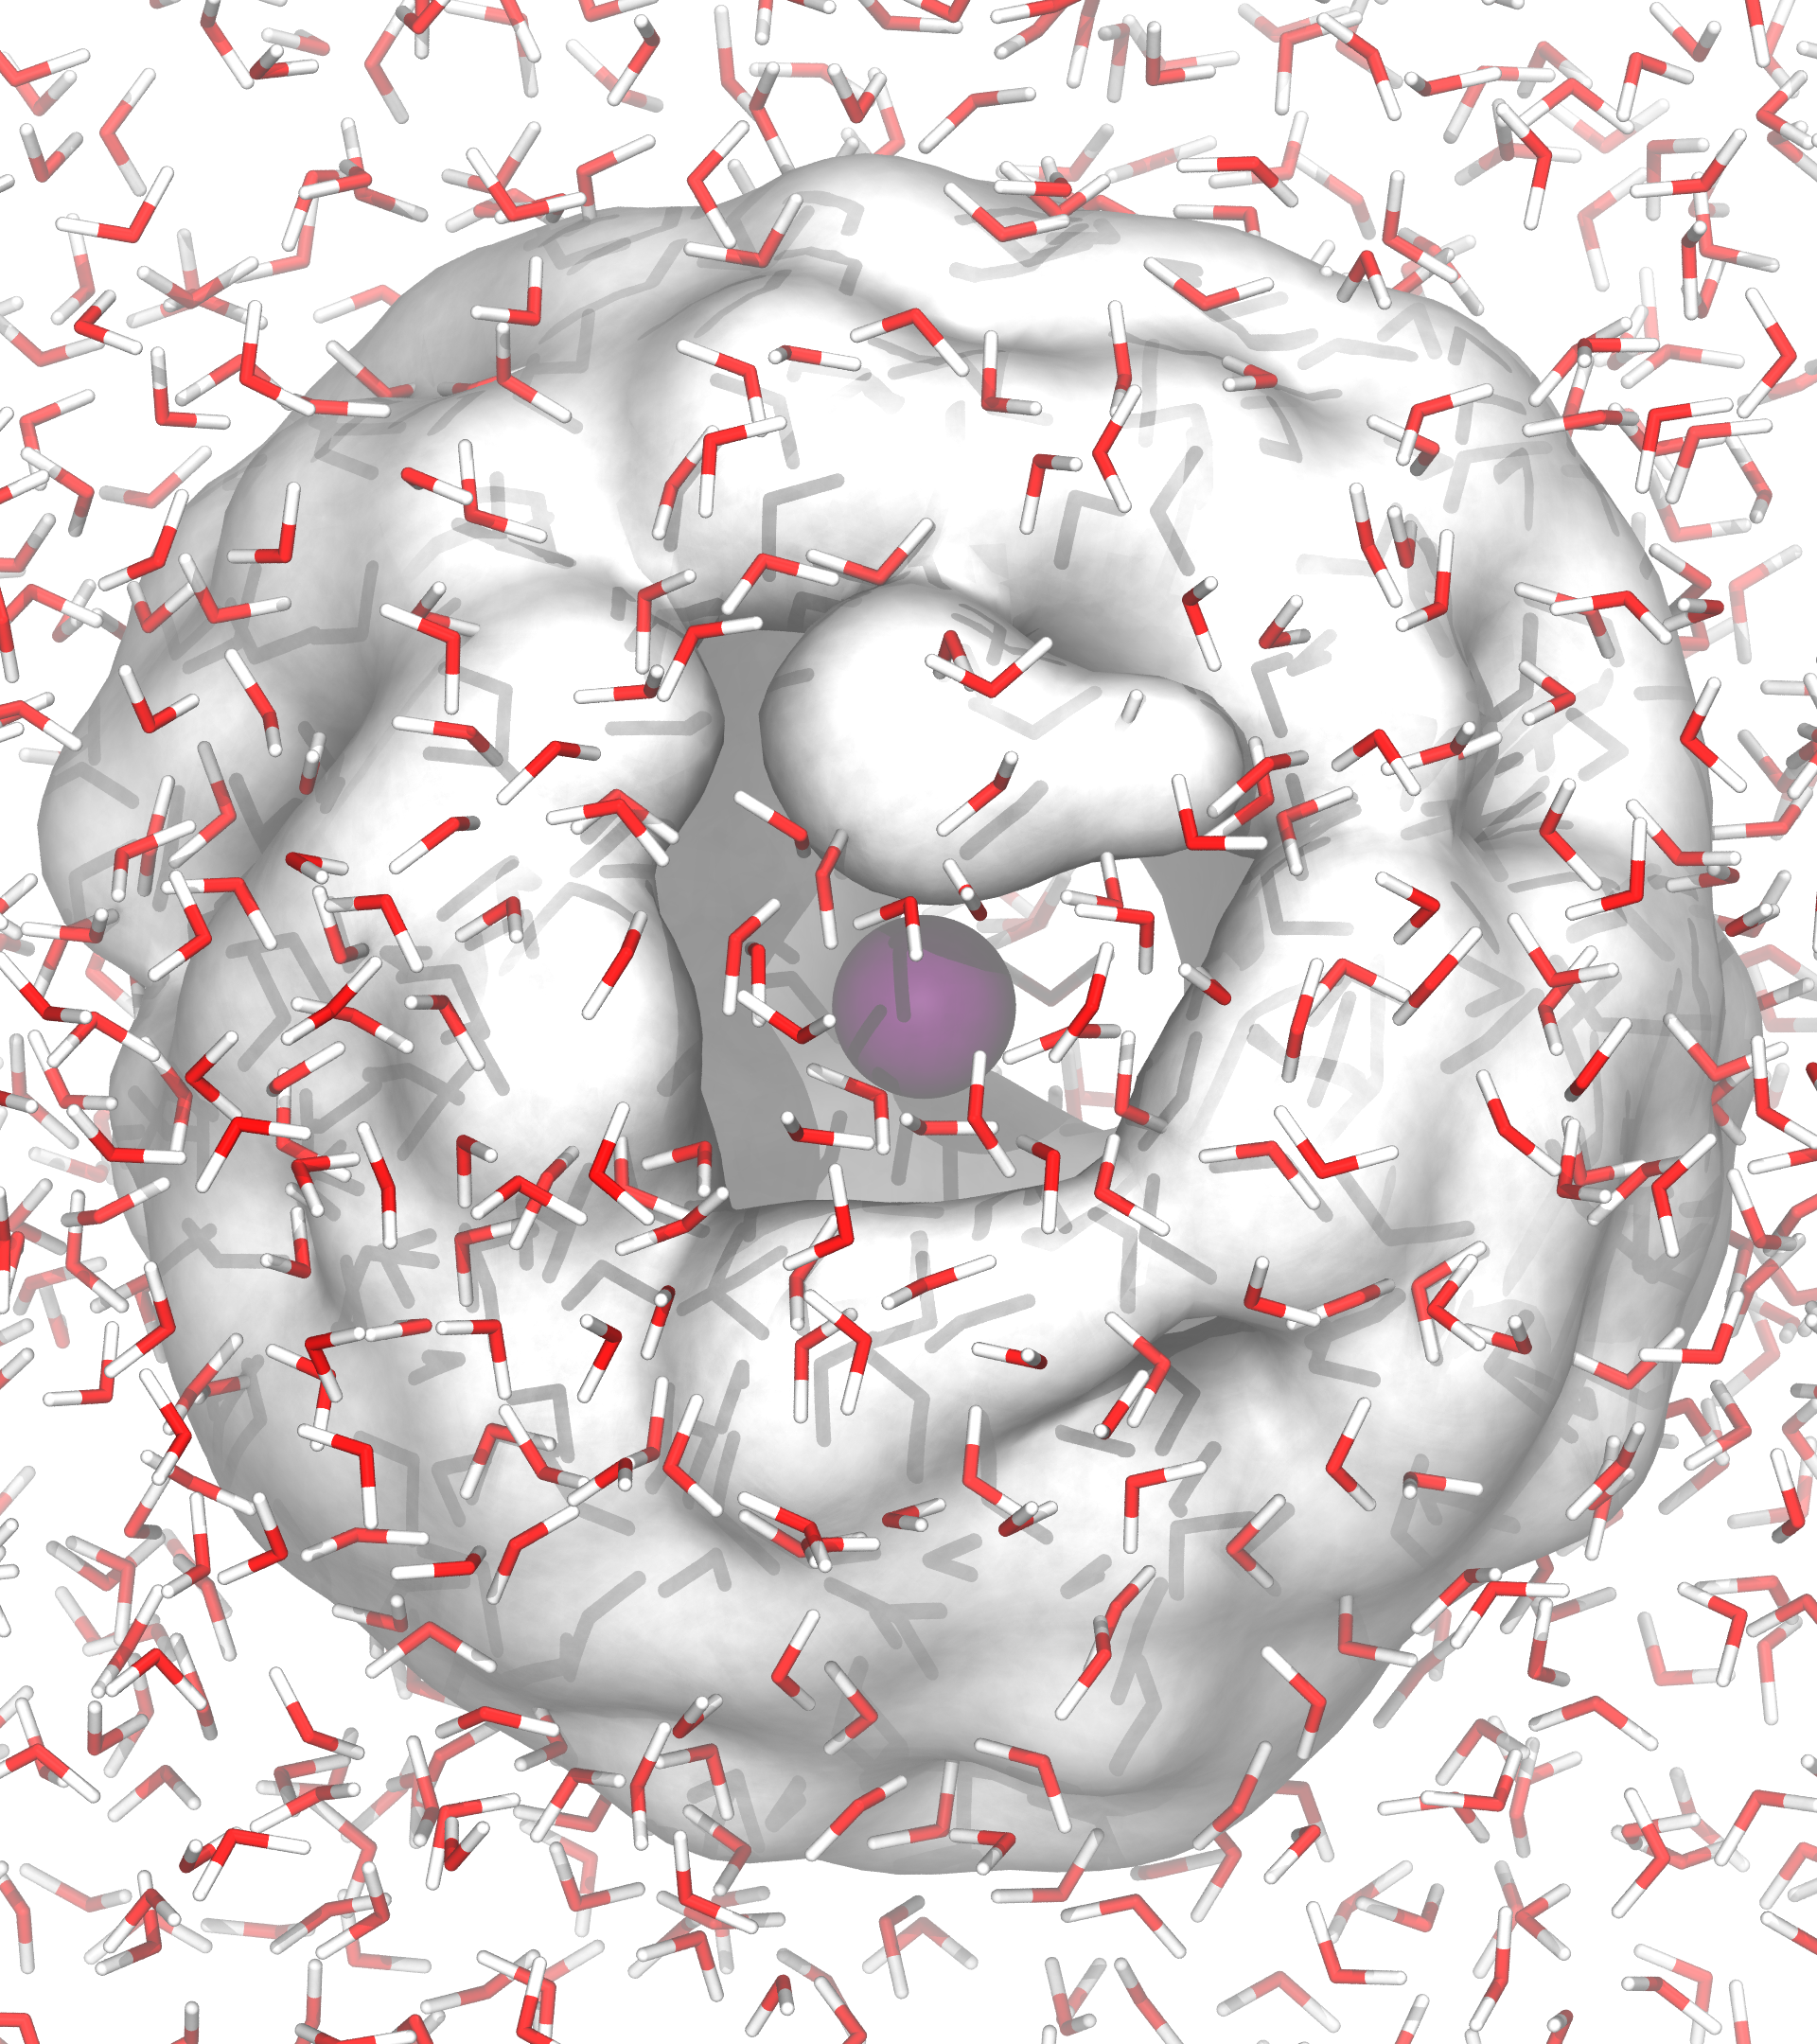
\includegraphics[width=0.30\linewidth]{images/tatb/wat.png}
  \includegraphics[width=0.30\linewidth]{images/tatb/dmso.png}
  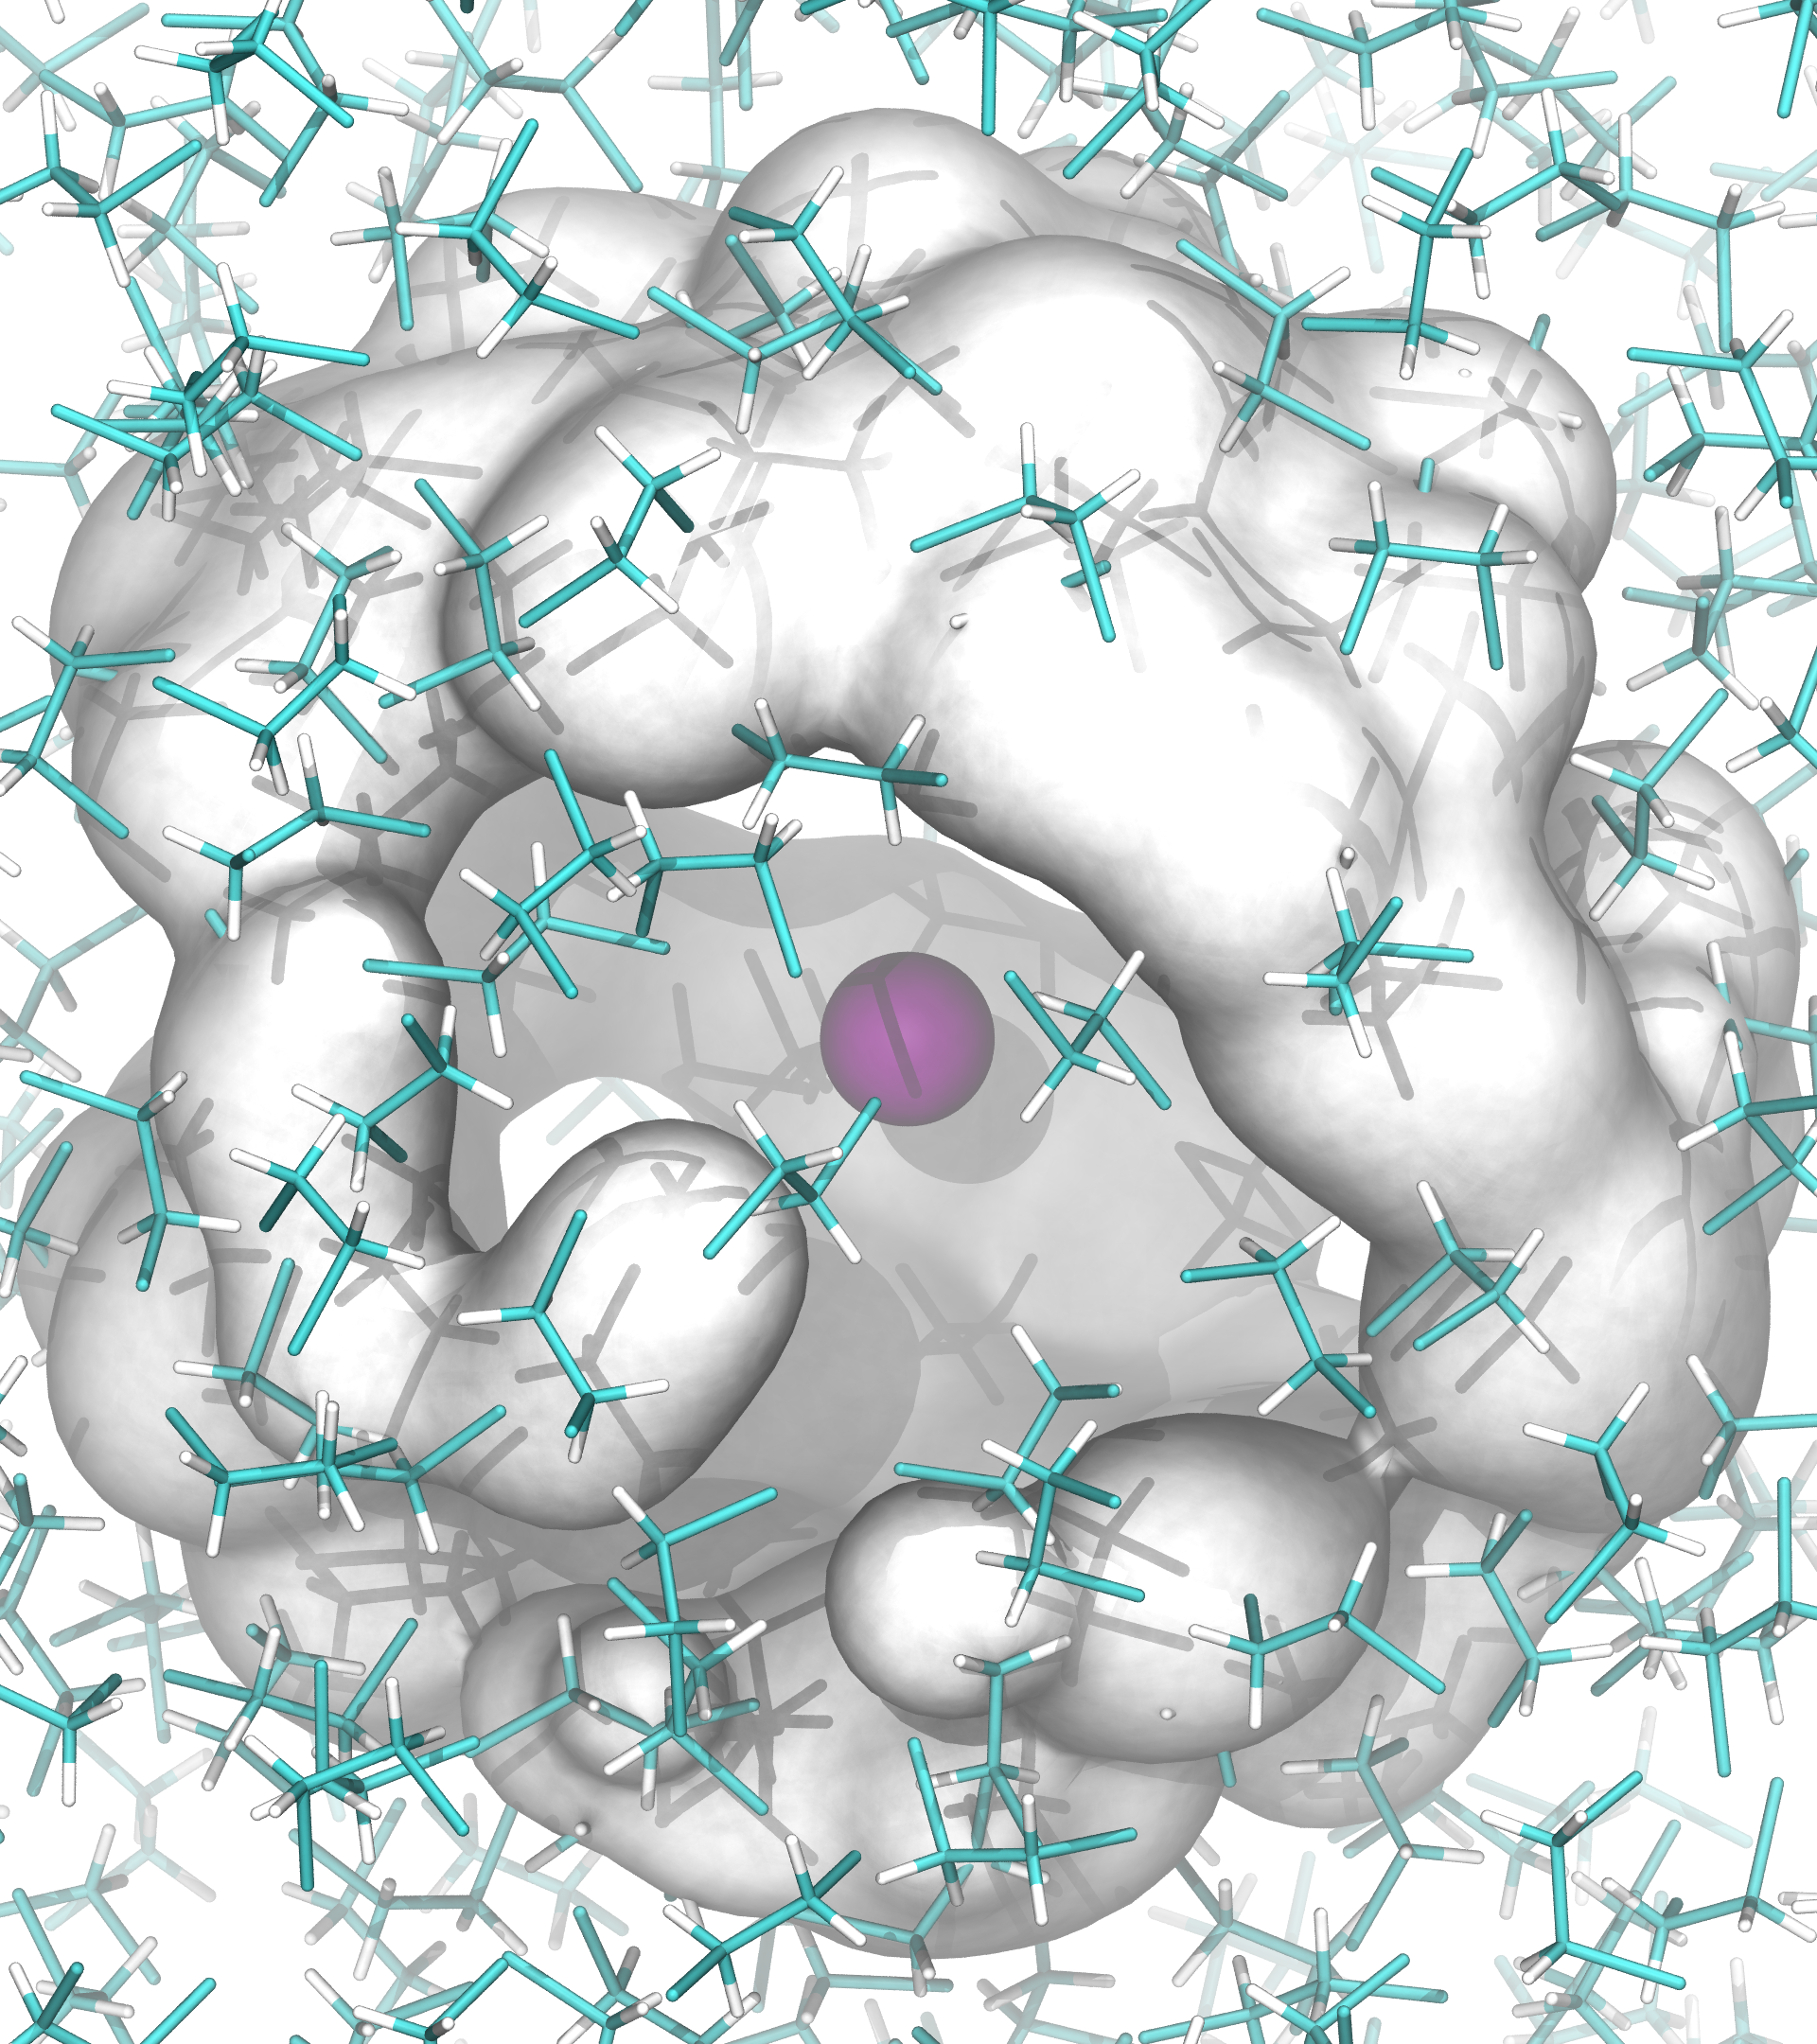
\includegraphics[width=0.30\linewidth]{images/tatb/dce.png}
  \caption[Snapshots of solvents with cavity volume excluded]{\label{fig:expelled_volume}Visualization of solvation structure at the boundary (white surface) 
  of the 0.90 nm radius cavity used to compute solvation free energies. The ion is at the center of this void, and is shown in purple. The solvents from left to 
  right are as follows: water, dimethyl sulfoxide, and 1,2-dichloroethane.}
 \end{center}
\end{figure}
 
  \section{\label{ch6:sec2:level1}Results~}

  \subsection{\label{ch6:sec2:level2}Packing and inner shell terms}
  I begin with some discussion of the cavity-related terms in each solvent: the packing and inner shell contributions. The packing free energy is independent of the 
  ion so I can very simply list the values for each solvent. For water this came out to 82.77 $\pm$ 0.63 kcal/mol which compares favorably with the result from Shi and
  Beck who produced a fit to a scaled-particle theory model\cite{shi2013length}. This value reflects the work required to clear a void of only the water oxygens since
  the hydrogens do not participate in the vdW potential. However, for both DMSO and 1,2-DCE, the hydrogens in these molecules have been assigned non-zero $\sigma$
  and $\varepsilon$ parameters. The cavity potential I used made no distinction between this atom or that based on mass and so acted the same on all particles provided 
  the force field recommended non-zero vdW parameters. A slightly larger value of 83.50 $\pm$ 0.91 kcal/mol was obtained for DMSO, while a much smaller result of 49.45
  $\pm$ 0.56 kcal/mol was found for 1,2-DCE. It's interesting to note that the cavity formation free energy in DMSO remains so large in spite of the pair of methyl 
  groups the solvent is forced to accommodate. Solvent/solvent contacts in 1,2-DCE however do appear to be relatively weak compared to both water and DMSO. Consequently, 
  the solvent is less tightly packed and so offers substantially less resistance to the insertion of large cavities and likewise to large, hydrophobic molecules and ions. 
  You can get a sense of this visually from Figure \ref{fig:expelled_volume} as well.

  A connection between the quasichemical packing contribution and the surface tension of the solvent was developed in Ref. \cite{shi2013length}. The surface tension for
  OPLS 1,2-DCE is 23.2 mN/m (expt 31.86 mN/m) while OPLS DMSO matches the experimental figure of 42.92 mN/m remarkably well (calc 42.4 mN/m)\cite{caleman2011force}. 
  Like 1,2-DCE, the surface tension of the SPC/E model (63.6 mN/m) is somewhat smaller than the experimental value (71.73 mN/m)\cite{vega2007surface}. Based on the model
  of Shi and Beck, I should still expect to see the packing contribution of water to be larger than DMSO, despite the smaller than expected SPC/E water surface tension.
  However, my finding is consistent with a scaled particle theory estimate from Abraham et al.\cite{abraham1979use}. Assuming the cavity term in Ref. \cite{abraham1979use}
  is positive too, then pack(DMSO) - pack(water) $>$ 0 means it costs more energy to put the cavity (here the cavity has a diameter of 0.84 nm) into DMSO. Their model
  appears to take into account the size of the solvent particles, which may account for the unexpected result.

  I continue the discussion focusing on Figure \ref{fig:inner}. For all ion $\sigma$ and $\varepsilon$ considered, the chemical part of the free energy showed that 
  the anion was better solvated in water and 1,2-DCE than the cation and generally followed the opposite trend in DMSO due to the hard S$=$O moiety. The gap between the 
  $\mu$\sursous{ex}{is} of complementary ions pairs (oppositely charged pairs with all other properties equal) diminishes to nearly zero for the largest radii in DMSO and
  water. This appeared to not be the case for ion solvation in 1,2-DCE where the charge-specific differences in smaller ion pairs remained essentially constant even when I 
  simulated TA\sur{+}/TB\sur{-}-sized particles. These results shed an initial favorable light on the validity of the TA\sur{+}/TB\sur{-} assumption in water and in DMSO as
  the large ions share nearly identical free energies in the ion specific region. A small amount of ion specificity is expected to survive based on the finite-size corrected
  fluctuation contributions in Figure \ref{fig:fq_flucts} which still show preference for one ion over the other, even using ions of TA\sur{+}/TB\sur{-} size. This hints 
  that the validity of the TA\sur{+}/TB\sur{-} assumption may rely on cancellation of lingering ion specificity by the $\phi$\sous{lp}.
  
\begin{figure} 
 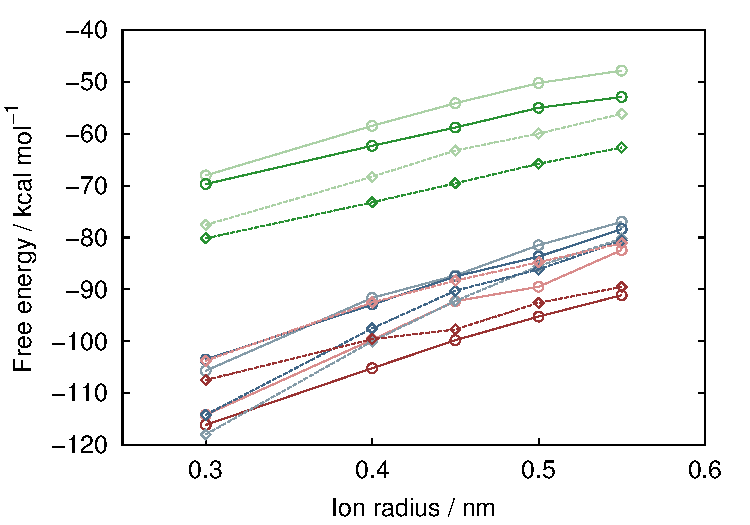
\includegraphics[width=0.98\linewidth]{images/tatb/is.pdf}
 \caption[Inner shell (chemical) part of the solvation free energy]{\label{fig:inner}Chemical or inner shell part of the solvation free energy for the ions in water
 (blues), dimethyl sulfoxide (reds), and 1,2-dichloroethane (greens). The darker shade corresponds to ions with $\varepsilon =$ 1.60 kJ/mol and the lighter shade for
 $\varepsilon =$ 0.16 kJ/mol. The cations are presented here with open circles at the sampled radii linked together with a solid line; anions at the sampled radii are
 represented as diamonds and are joined together with dashed lines. Error bars are omitted as they are about the same size as the symbols and are reported in the tables
 in Appendix \ref{chap:a6}.}
\end{figure}

\begin{figure} 
 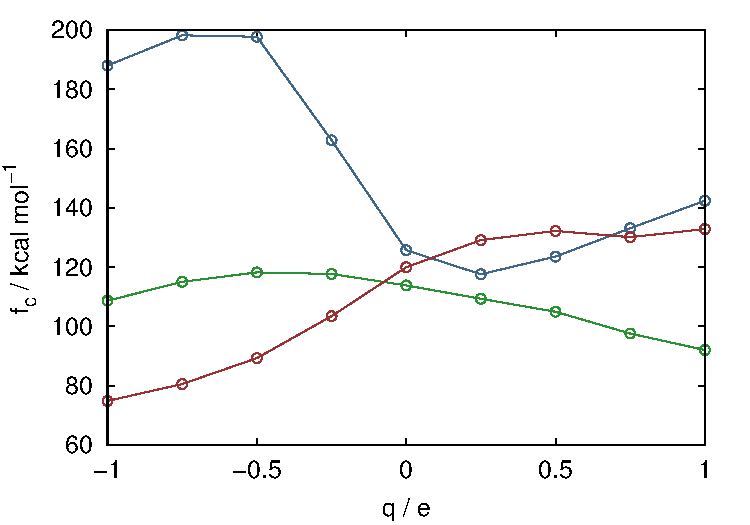
\includegraphics[width=0.80\linewidth]{images/tatb/cl_sized_fq_var.pdf} \\
 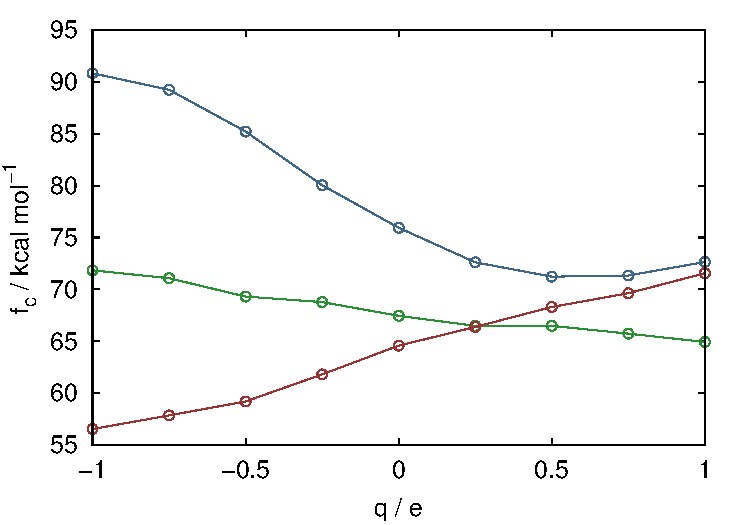
\includegraphics[width=0.80\linewidth]{images/tatb/tatb_sized_fq_var.pdf} 
 \caption[Corrected fluctuations of the electrostatic potential at the center of an uncharged cavity]{\label{fig:fq_flucts}Finite-size corrected fluctuations of
 the electrostatic potential at the center of the Horinek and Netz Cl\sur{-}-ion (top) and a TA\sur{+}/TB\sur{-}-ion (bottom). Figures are reported as solid lines 
 in blue for water, red for DMSO, and green for 1,2-DCE.}
\end{figure}

  \subsection{\label{ch6:sec2:level3}Outer shell and local potential terms}
  I begin this section with some discussion of the motivations for electing to use the mid-point approximation to the outer shell free energy. Normally, I would sample
  the fully coupled interaction energies from the final $\lambda$ state in both the packing (uncoupled) and inner shell (coupled) trajectories. However, as pointed out
  by Shi and Beck\cite{shi2013length}, there needs to be continuity in the solvation environment between that sampled with $\pm$q and a neutral but otherwise identical
  particle. Monitoring the mean-field part of the electrostatic potential at the center of a cavity bearing integer and fractional charges in the range of -q to q is a
  particularly useful way for interrogating the solvation shell for charge-specific asymmetries, see Figure \ref{fig:fq_means}. As noted by Wipff et al., the water dipole
  orientation around the
  neutral cavity more resembles the solvation environment around a positively charged ion\cite{wipff1999tatb}. Unsurprisingly, I found the mean-field part of the
  electrostatic potential for the neutral particle fell on the same line drawn through the points with positive charge. The same observation was made from the
  TA\sur{+}/TB\sur{-}-sized ion data set as well. Lines through the negatively and positively charged ion data intersect at -0.22e and -0.17e for the smaller and larger
  ion sizes, respectively. The deviation between these lines is reduced with the larger particles, but not enough to allay concerns over errors introduced by sampling
  energies from dissimilar solvation environments. I've found likewise in DMSO as well, where the lines intersect at -0.16e and -0.11e. In contrast, the solvation
  environment around the neutral cavity in 1,2-DCE slightly favored the anion and produced intersections at 0.22e and 0.03e. An additional point, the potential at the
  center of the neutral cavity can be taken as a crude estimate of $\phi$\sous{lp}, with some caveats discussed below.
  
\begin{figure}
 \begin{center}
  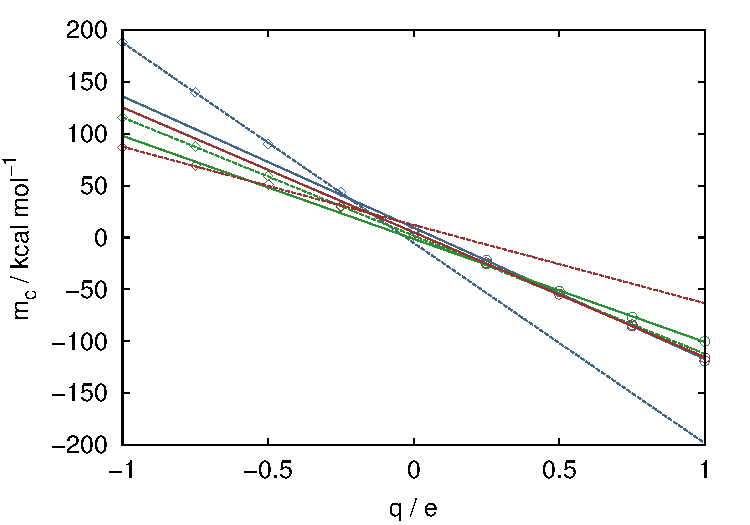
\includegraphics[width=0.80\linewidth]{images/tatb/cl_sized_fq_means.pdf} \\
  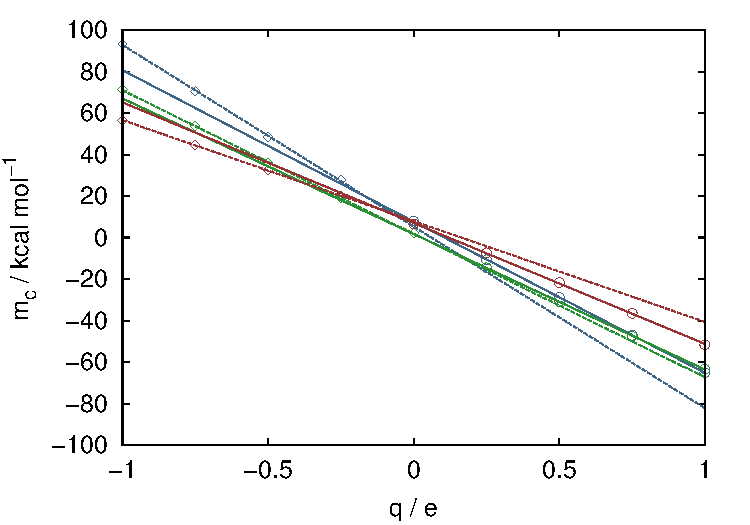
\includegraphics[width=0.80\linewidth]{images/tatb/tatb_sized_fq_means.pdf}
  \caption[Corrected mean of the electrostatic at the center of an uncharged cavity]{\label{fig:fq_means}Finite-size corrected means of the electrostatic
  potential at the center of the Horinek and Netz Cl\sur{-}-ion (top) and a TA\sur{+}/TB\sur{-}-ion (bottom). Colors correspond to solvents: blue for water, red for
  DMSO, and green for 1,2-DCE. A dashed line is used to show the linear fit through the negatively charged points and a solid line for the fit through the neutral and
  positively charged data points.}
 \end{center}
\end{figure}

  The mid-point approximation for $\mu$\sursous{ex}{os} provides a straightforward decomposition pathway to separate vdW and electrostatic sources as in Equation 
  \ref{eqn:os}. Assuming any differences in the vdW energy between the ions to be small, the top plot in Figure \ref{fig:outer} depicts the results from the cumulant
  expansion of the electrostatic contributions to $\mu$\sursous{ex}{os}. Across the range of ion radii covered here and in all solvents, this plot shows a very nearly
  constant gap between the complementary sets of ions. I argue this gap is due to the presence of a q$\phi$\sous{lp} factor for each ion. As the bottom plot in 
  Figure \ref{fig:outer} illustrates, the removal of this factor shifts the free energy differences into near perfect overlap with some residual due to non-Gaussian
  behavior in the vdW contributions for the organic solvents. The electrostatic contributions are within 0.5 kcal/mol of each other across 3 separate trajectories
  with small differences in the variance and higher order terms. A slightly larger cavity may be needed for DMSO and 1,2-DCE to remove the remaining small, but not 
  insignificant non-Gaussian behavior.

\begin{figure}
 \begin{center}
  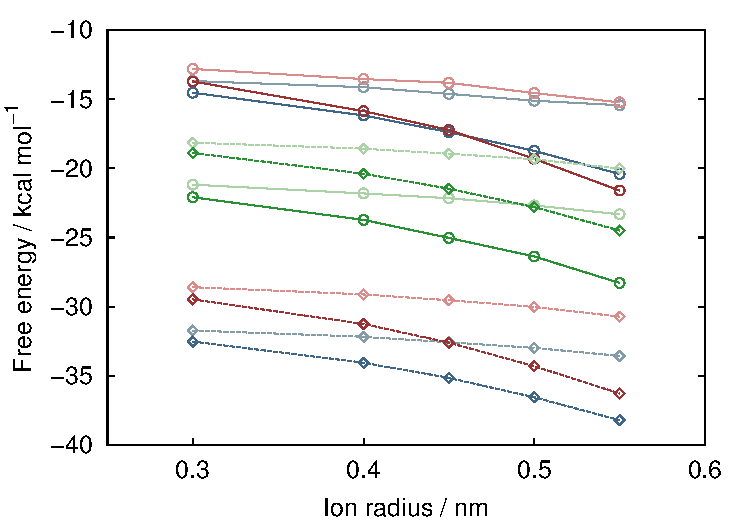
\includegraphics[width=0.80\linewidth]{images/tatb/os.pdf}
  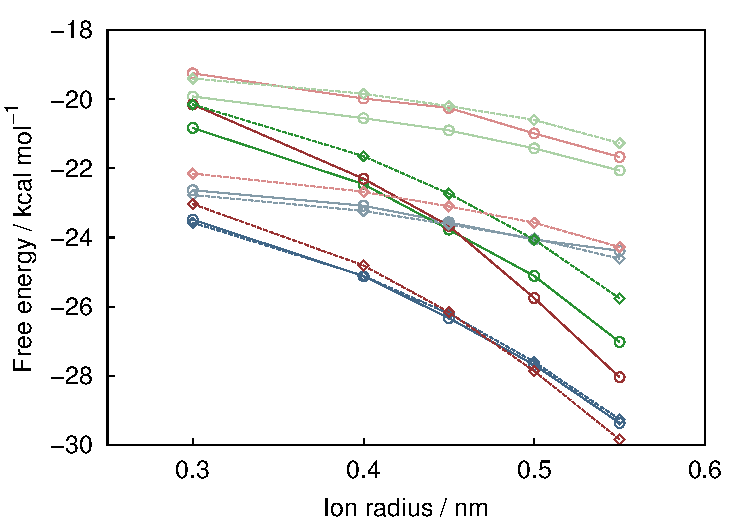
\includegraphics[width=0.80\linewidth]{images/tatb/os_m_qlp.pdf}
  \caption[Outer shell portion of the solvation free energy]{\label{fig:outer}Full outer shell (top) and outer shell less the local potential (bottom) part of the
  solvation free energy. Color and labeling scheme are the same as described in Figure \ref{fig:inner}.}
 \end{center}
\end{figure}

  The local potential in each solvent [in (mean + third cumulant); total $\pm$ error format] was determined to be (8.76 + 0.20); 8.95 $\pm$ 0.14 kcal/mol-e, 
  (6.71 + -0.27); 6.44 $\pm$ 0.24 kcal/mol-e, and (-1.42 + 0.16); -1.26 $\pm$ 0.20 kcal/mol-e in water, DMSO, and 1,2-DCE respectively. These potentials were sampled
  from configurations generated with an empty 0.9 nm radius cavity buried in each solvent. The potential makes no distinction between light and heavy atoms so long as
  they are described with non-zero terms in the conventional LJ function, else those atoms are ignored for consistency with the force field. This method was shown by
  Ashbaugh to produce well-converged results at the same length scale I used here\cite{ashbaugh2000size_sp}. Simply using the neutral point in the fluctuating 
  electrostatic potential calculations discussed previously can, in some cases, net you a fortuitously close result, but it displays significant size variance and may
  even predict the wrong sign for solvents with smaller $\phi$\sous{lp}. This is a consequence of using standard LJ interactions in the simulation which operate on 
  different length scales for each atom type, so smaller elements tend to settle a bit closer to the ion than they would with my modified WCA potential, for example.
  The local charge balance at the cavity is skewed in favor of the charge of these smaller elements, usually hydrogens. The positive charge on these atoms introduces an 
  artificial shift driving $\phi$\sous{lp} more positive, or negative as the case may be. A similar shift occurs when applying the cavity-growth potential to hydrogens 
  in the SPC/E or other single vdW-site water models and actually yields a $\phi$\sous{np} around -0.4 V, though this is almost assuredly coincidental\cite{beck2013sp}.

  \subsection{\label{ch6:sec2:level4}Free energy differences}
  I now have all the pieces needed to assemble the total solvation free energies and examine how the differences between the ions transition with increasing size. 
  These values are reported in Appendix \ref{chap:a6} in a tabular format complete with error bars for both the intermediate and bulk free energy scales. The 
  differences between the single-ion solvation free energies listed in those tables are depicted in Figures \ref{fig:uex_diffs1}, \ref{fig:uex_diffs2}, and 
  \ref{fig:uex_diffs3}. Where appropriate I have included figures taken from Wipff et al.\cite{wipff1999tatb} and Pliego et al.\cite{pliego2015ccqct} to highlight not
  only my agreement with these additional studies but to showcase that their respective results fall on very different thermodynamic scales and lead to very different
  conclusions. Removal of q$\phi$\sous{lp} from $\mu$\sursous{ex}{os} extinguishes the artificial stabilization of anions relative to their cation analogue in both 
  SPC/E water and OPLS/AA DMSO that produced the $\sim$20 kcal/mol disparity in TB\sur{-} versus TA\sur{+} solvation free energies reported by Schurhammer and Wipff.
  Withdrawing q$\phi$\sous{lp} from $\mu$\sursous{ex}{os} in 1,2-DCE created a slightly greater rift in the ion solvation free energies with a deviation from ideal
  behavior of about 6-10 kcal/mol in favor of the anion. This range is similar to that of acetonitrile as discussed by Pliego et al.\cite{pliego2015ccqct}.  

\begin{figure} 
 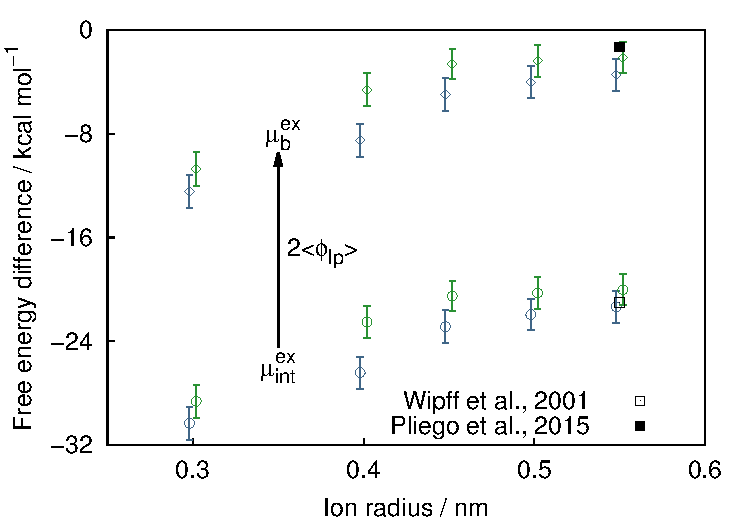
\includegraphics[width=0.98\linewidth]{images/tatb/wat_free_energy.pdf}
 \caption[Free energy differences in water]{\label{fig:uex_diffs1}Free energy differences in complimentary ion pairs in water. Open circles represent 
 intrinsic free energy points while open diamonds are on the bulk free energy scale. Blue coloring corresponds to ions with $\varepsilon =$ 0.16 kJ/mol 
 while green marks $\varepsilon =$ 1.60 kJ/mol differences. Where appropriate, comparisons to the Wipff and Pliego results are reported.}
\end{figure}

\begin{figure} 
 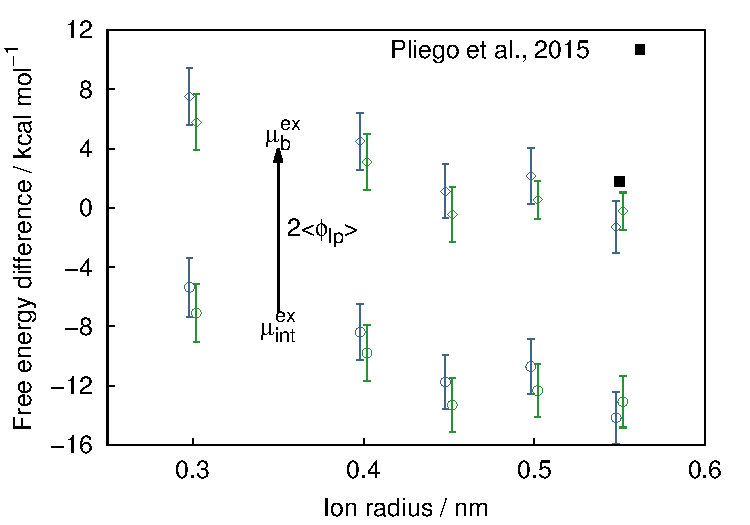
\includegraphics[width=0.98\linewidth]{images/tatb/dmso_free_energy.pdf}
 \caption[Free energy differences in dimethyl sulfoxide]{\label{fig:uex_diffs2}Free energy differences in complimentary ion pairs in DMSO. Open circles 
 represent intrinsic free energy points while open diamonds are on the bulk free energy scale. Blue coloring corresponds to ions with $\varepsilon =$ 0.16 
 kJ/mol while green marks $\varepsilon =$ 1.60 kJ/mol differences. Where appropriate, comparisons to the Wipff and Pliego results are reported.}
\end{figure}

\begin{figure} 
 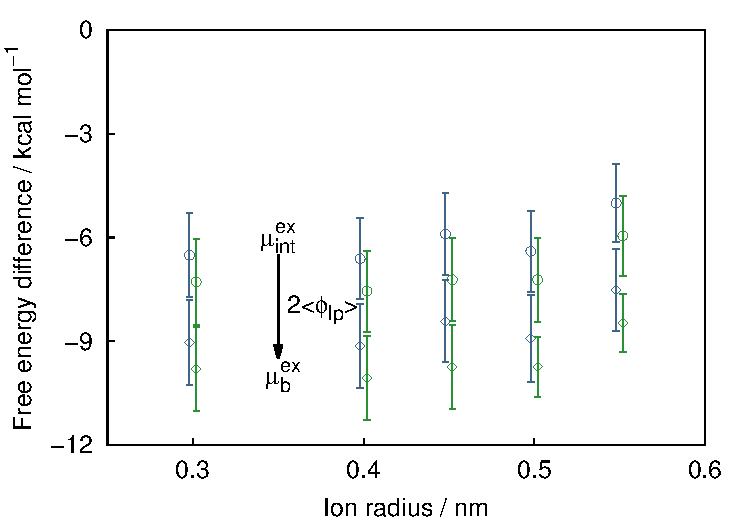
\includegraphics[width=0.98\linewidth]{images/tatb/dce_free_energy.pdf}
 \caption[Free energy differences in 1,2-dichloroethane]{\label{fig:uex_diffs3}Free energy differences in complimentary ion pairs in 1,2-DCE. Open circles 
 represent intrinsic free energy points while open diamonds are on the bulk free energy scale. Blue coloring corresponds to ions with $\varepsilon =$ 0.16 
 kJ/mol while green marks $\varepsilon =$ 1.60 kJ/mol differences.}
\end{figure}

  \section{\label{ch6:sec3:level1}Discussion~}
  Qualitatively, the result that anions are more strongly hydrated than cations falls in step with a number of other studies\cite{wipff1999tatb, pliego2015ccqct,
  ren2003amoeba, collins2007review, collins1995}. Assuming the F\sur{-} and K\sur{+} ions to be of nearly identical size (or perhaps more conservatively, between
  Na\sur{+} and K\sur{+})\cite{wright2010ionsize}, Rose et al. also concluded that the anion interacted more favorably with 1,2-DCE than the cation\cite{rose2009}. 
  And finally, in agreement with the somewhat dated conductometric studies of Exner et al.\cite{exner1974dmso} and more recent simulation results of Pliego et al. for
  intermediate\cite{pliego2002dmso} and bulk free energies\cite{pliego2015ccqct}, I found the cation produced a larger $\mu$\sur{ex} part than its complementary anion. A
  more quantitative assessment of the accuracy of my results was a bit more difficult to come by, but the extensive work of Abraham et al. (Table 8)\cite{abraham1978} 
  allowed me to get an approximate sense of where my bulk free energy results fell for the more physically motivated ion parameter sets (cations with $\varepsilon
  =$ 0.16 kJ/mol and anions with $\varepsilon =$ 1.60 kJ/mol). For example, I properly recovered that the transfer free energy from water to 
  1,2-DCE was unfavorable for smaller ions, up to the size of tetraethylammonium (TEA\sur{+}) which has an ionic radius in the neighborhood of 0.3 to 0.4 
  nm\cite{aue1976tea}. Given the trend reported in their article and second harmonic generation spectroscopic investigation of the water/1,2-DCE 
  interface\cite{conboy1997shg_tatb}, I know that larger ions eventually become better suited to the oil over water. Likewise, the cation solvation free energies in
  DMSO were found to be greater than that in water which was also observed by Pliego et al.\cite{pliego2002dmso}. For anions, the smallest one gave a positive transfer 
  free from water to DMSO consistent with these other authors but beyond that reverses. Within the limitations of the force field, these results compare rather favorably
  against other studies, but it is important to note the parameters used here were not designed to handle ion solvation problems. They neglect or oversimplify difficult
  to characterize polarization and partial charge transfer contributions\cite{pollard2016review}, which can be difficult to overcome even when fitting some of the parameters
  to high level electronic structure calculations\cite{ayse2016ecpc}. Above all though, this exercise is meant to be illustrative of a broader concern and even the
  poorest force fields are susceptible to these interfacial potential issues.

  In Table 4 of the Wipff manuscript for the spherical S\sur{+} and S\sur{-}, the authors show that the electrostatic part of the interaction energy favors the anion
  by 23 kcal/mol\cite{wipff2000tatb}. This difference is also reflected in Table 5, where they report the electrostatic potentials at the center of both charged and
  uncharged solutes\cite{wipff2000tatb}. The mean electrostatic potential at the center of the uncharged S\sur{0} particle with a radius of 0.55 nm was found to be 7.4
  kcal/mol with TIP3P water. This figure is similar to that reported by Ashbaugh at the same distance in SPC/E water\cite{ashbaugh2000size_sp}. This is $\phi\sous{lp}$,
  albeit with too small a cavity. The authors do not remove this contribution from the figures reported in Table 2\cite{wipff2000tatb}. With a positive $\phi\sous{lp}$,
  the -21.0 kcal/mol $\Delta\mu^{ex}$ is increased by +14.8 kcal/mol to give a difference of -6.2 kcal/mol which compares favorably against my own figure.

  As a point of comparison, the $\phi\sous{lp}$ reported for TIP5P is much smaller, on the order of about 1 kcal/mol-e\cite{wipff2000tatb}. TIP5P water has been observed
  by Mundy et al.\cite{remsing2014lp} and Ichiye et al.\cite{ichiye2015sp} to exhibit rather unusual behavior in relation to the ongoing dialogue about the conventional
  surface potential, $\phi\sous{sp}$, and the electrochemical surface potential, $\phi\sous{np}$. Recently, Pollard and Beck calculated the latter, $\phi\sous{np}$, felt
  by a charge in water to be -0.4 V\cite{pollard2014cpa1, pollard2014cpa2}. Water models such as TIP3P and SPC/E underestimate this potential somewhat, but the
  potential from TIP5P is very nearly zero. This is because the quadrupole and octupole moments of the TIP5P water model compare poorly against the experimental and
  \emph{ab initio} predicted  values\cite{niu2011large}. Though an exact relationship between the quadrupole moment (and higher order moments) is unknown, 
  $\left|\phi\sous{sp}\right|$ has been found to be proportional to the quadrupole moment of the water model for the basic point charge models 
  (i.e., TIPXP, SPC, SPC/E)\cite{ichiye2015sp}. Note, that the SSDQO model which does not follow the trend in the Ichiye et al. paper also incorporates oxygen-centered
  point dipoles, quadrupoles, and octupoles.

  With respect to the TA\sur{+}/TB\sur{-} hypothesis, I found a 2.13 kcal/mol deviation from cation/anion solvation parity in SPC/E water. The error bars include 1.28
  kcal/mol prediction of Pliego et al.\cite{pliego2015ccqct} who combined gas phase electronic structure calculations at the MP2 and MP4 levels of theory with continuum
  solvation using the SMD model. Their results found a similarly small deviation from the TA\sur{+}/TB\sur{-} scale in DMSO of 1.8 kcal/mol which fell just outside the
  error bars of my result. A key tenet of the TA\sur{+}/TB\sur{-} hypothesis is that such ions give the same solvation free energy in \emph{every} solvent. Calculations
  in acetonitrile, however, revealed a nearly 10 kcal/mol shift from TA\sur{+}/TB\sur{-} behavior. I observed a comparable disparity in the solvation free energies on
  the bulk/Marcus scale in 1,2-dichloroethane spurred by the solvation asymmetry in the inner shell term favoring the anion and a negative $\phi\sous{lp}$ which further
  separated $\Delta\mu\sur{ex}(X\sur{+}\rightarrow X\sur{-})$.

  \section{\label{ch6:sec4:level1}Conclusions~}
  I have presented a case that simulations of ionic species even in periodic boundary conditions with no vapor region include a potential centered about the ion.
  The potential is the product of broken multipolar symmetry relative to the bulk. It also impacts the solvation free energy, solvation enthalpy, and related
  properties such as pKa of charged species. The local potential is solvent dependent but applies in increments of $\pm$q, where q is the ion charge. Difficulties in
  the development of proper force fields for divalent cations like Mg\sur{2+} and Ca\sur{2+} may in part owe some of their trouble to the mishandling of this 
  potential which would impart a $\sim$18 kcal/mol error in $\mu\sur{ex}$ and h\sur{ex} (assuming $\frac{\partial\phi\sous{lp}}{\partial T} \approx 0.~$V, same physical
  origin as $\phi\sous{sp}$\cite{gabdoulline1997mean}) in SPC/E  water. Also of note, the TA\sur{+}/TB\sur{-} scale agrees with other surface potential free (\emph{bulk scale})
  methods such as quasichemical theory\cite{asthagiri2003absolute,asthagiri2004hydration,pollard2014cpa1}, the Latimer-Pitzer-Slansky model with re-fit ionic 
  radii\cite{ashbaugh2008lps}, and a second set of values predicted by Marcus with a model similar to that of Born\cite{marcus1985book}.
  
  I've also re-examined the tetraphenylarsonium/tetraphenylborate assumption which postulates that oppositely charged ions in a large, shielding ligand network have 
  the same solvation free energy in every solvent. Previous work had shown the anion of this pair to be on the order of $\sim$20 kcal/mol more strongly hydrated than
  the cation. I showed this difference reflected the influence of a factor of q$\phi$\sous{lp} for each ion and that these ions possessed nearly identical free
  energies in the absence of the potential. I also managed to extend the analysis to dimethyl sulfoxide (DMSO) and 1,2-dichloroethane (1,2-DCE) using the OPLS/AA 
  force field. It was found that DMSO behaved similarly to water, where removing the potential allowed me to compare favorably against a recent continuum model
  investigation, while 1,2-DCE violated this assumption even after removing $\phi$\sous{lp}. I concluded that the assumption was possibly valid in water and DMSO
  despite the model deficiencies thanks to my excellent comparison to MP4 level quantum chemistry calculations by Pliego and coworkers. Finally, it is my opinion 
  that these interfacial potentials have profound and far reaching implications in the world of force field optimization. However, I discuss in detail a road map 
  for how to go about comparing existing force field results to experiment.
  
  \vspace{12 pt}
  
  \begin{wbepi}{Futurama}
   Leela: ``Five thousand feet!'' \\
   Farnsworth: ``Dear Lord! That's over one hundred and fifty atmospheres of pressure.'' \\
   Fry: ``How many atmospheres can the ship withstand?'' \\
   Farnsworth: ``Well, it's a space ship. So I'd say anywhere between zero and one.''
  \end{wbepi}

\end{tatb}